\chapter{Preparation}

\section{Theory}


\section{Preparation Questions}

\subsection{Question 1}
\begin{figure}[ht]
\centering
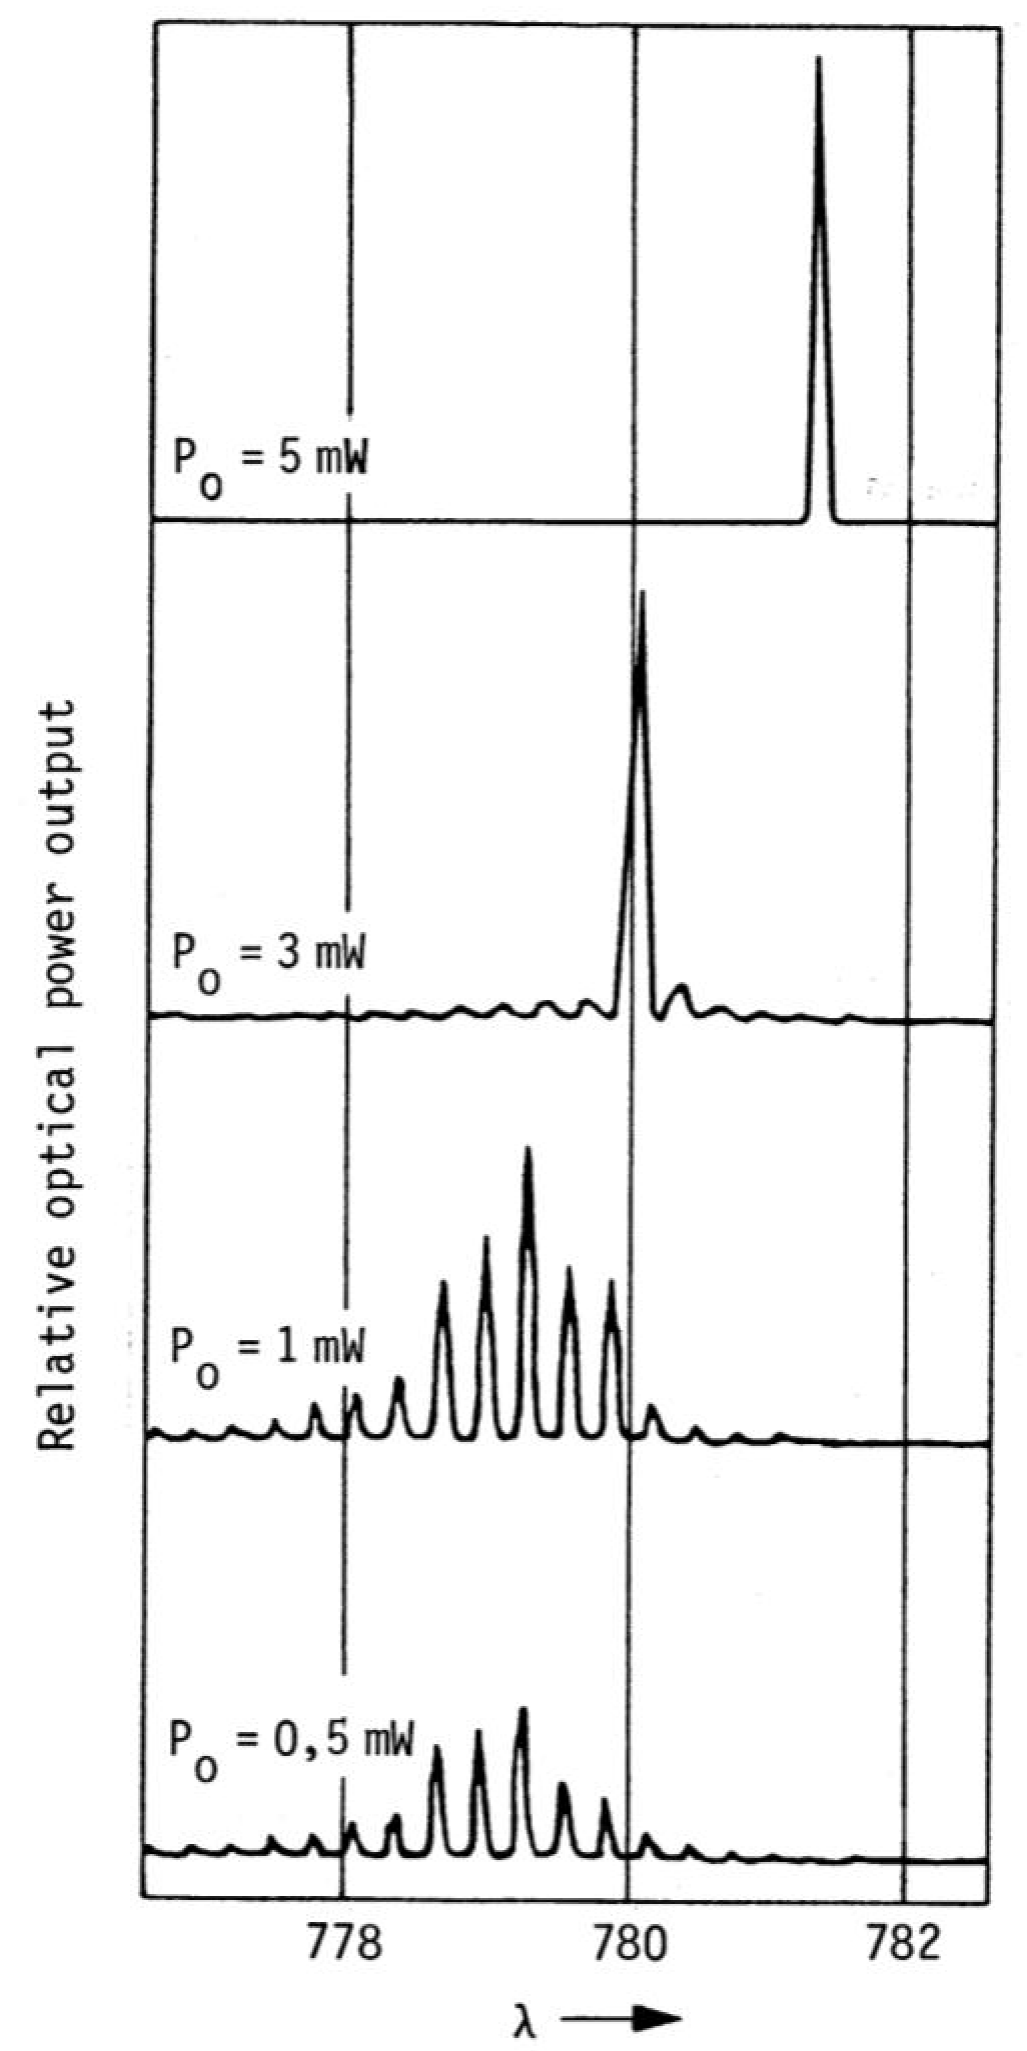
\includegraphics[width=.3\columnwidth]{Grafiken/Q1.png}%
\caption{output spectra of a laser diode for different optical output powers.}%
\label{fig:Q1}%
\end{figure}
The output spectra of a laser diode is shown in figure \ref{fig:Q1}\footnote[1]{Optical Communications Lab - Experiment 1, Preparation Materials} for different output powers $P_0$. 
There are different modes in the output spectrum.  How much modes exist depends on the optical gain each mode experiences. For a low output power the the spectrum is multimoded, for a higher power it gets single mode.\footnote[2]{Optoelectronics and Photonics; S. O. Kasap; Prentice Hall, 2001}
For a low output power several modes can be amplified by the material. For higher powers, all electrons are involved in the amplification of the one mode. The other modes can't be amplified any more.
\comwo{sehr komische sache, ne quelle wos drinsteht w�r gut}
 
For higher powers the spectrum of the laser shifts to a longer wavelength.
An applied current through the flows nearly complete through the active zone of the laser diode. Because the refractive index depends on the carrier density\footnote[3]{Optische Nachrichtentechnik; Grau, G.; Freunde, W.; 3. ed.; Springer 1991} it changes with higher currents and therefore with higher optical output powers.

Since the resonance frequencies of the laser depend on the refractive index of the material, the frequencies shift with the higher output power as well.

\todo{nochmal kontrollieren, und warum �ndert sich der optical gain auch mit der leistung? sicher auch wegen $\Delta n$.}



\subsection{Question 3}

With the free spectral range
\begin{equation}
 \Delta f\i{q}
\end{equation}


\subsection{Question 5}
\subsubsection{5. a)}

\begin{equation}
\frac{dN_p}{dt}=\left[ \Gamma G(n_T) - \frac{1}{\tau_p} \right] + \Gamma G(n_T)n_{sp}(n_T)
\label{eq:}
\end{equation}
There are different parts in the differential equation with different physical meanings.

\begin{itemize}
	\item $\frac{dN_p}{dt}$ is the change of the number of photons per time.
	\item $N_P \Gamma G(n_T)$ are the through stimulation generated photons per time.
	\item $-\frac{N_P}{\tau_p}$ are the outcoupled and absorbed photons per time.
	\item $\Gamma G(n_t)n_{sp}(n_t)$ are the spontaniously generated photons per mode and time.
\end{itemize}

and in

\begin{equation}
\frac{d(n_T V_r)}{dt} = \frac{I}{e}-r_{eff}(n_T)V_R-N_P\Gamma G(n_t)
\label{eq:}
\end{equation}


\begin{itemize}
	\item $\frac{d(n_T V_r)}{dt}$ is the change of the number of electrons per time.
	\item $\frac{I}{e}$ are the injected electrons per time
	\item $-r_{eff}(n_T)V_R$ are the spontaneous and non radiative depleted electrons per time.
	\item $-N_p\Gamma G(n_T)$ are the through stimulation depleted electrons per time.
\end{itemize}